\begin{onehalfspace}
\section{Motivation}
\subsection{Problemstellung}
\label{s:intro}
Das übergeordnete Ziel für die Bausoftware ORCA AVA ist es, möglichst viele Informationen aus 3D-Modellen von Gebäuden in der Ausschreibungssoftware automatisch importieren zu können. Das spart dem Architekten am Anfang in der Ausschreibung viel Zeit. Der für die Bachelorarbeit relevante Teil ist die Übernahme der Baustoffe und Materialien des Objektes/Bauteils. Aus dem Modell übernommene Bauteile sollen also automatisch einer im vor hinein generierten Material-Kostengliederung zugewiesen werden.
Als öffentliches Standardformat für 3D-Gebäudemodelle gibt es IFC, welches auch in der ORCA AVA benutzt wird. In diesen Modellen können auch die Materialien der einzelnen Bauteile spezifiziert werden. Diese können an verschiedenen Stellen an einem Bauteil im Modell angegeben werden. Für Materialbezeichnungen gibt es auch keine richtigen Standards. Hier besteht das Problem, dass das Textfeldern für die Materialangabe ein offenes Textfeld ist und somit keine feste Vorgabe existiert und jedes IFC-Modell anders strukturiert ist. Deswegen ist das Ergebnis jeder Kostengliederung unterschiedlich und vom jeweiligen Modell abhängig.

\subsection{Ziel}
Ziel ist es eine Kostengliederungsstruktur in der Bausoftware ORCA AVA aus den Materialeininformationen einer IFC-Datei zu generieren. Diese Kostengliederung kann am Anfang eines Projektes einmal importiert werden. Wenn dann im Laufe des Ausschreibungsprozesses ein Bauteil aus der IFC-Datei in die ORCA AVA übernommen wird, soll es automatisch einem Material in dieser Kostengliederungsstruktur zugewiesen werden. So kann man das ausgeschriebene Gebäude nach den Materialangaben sortieren und auswerten.
\\


Ein Algorithmus soll zuerst die Möglichkeiten der Materialangabe in der IFC-Datei zusammenführen. Mit Hilfe von Natural Language Processing und Artificial Inteligence eine Lösung entwickelt werden, um einen klassifizierten und standardisierten Materialbaum zu erschaffen. Dieser Baum muss am Ende in das schon von ORCA vorhandene Format einer Kostengliederung abgebildet werden.


\section{Ausgangslage}

Das Projekt basiert vor allem auf das Themengebiet von Natural Language Processing (NLP). Mit Algorithmen wie WordNet oder Textklassifizierungen.

Innerhalb der Firma gibt es noch fast kein Wissen über dieses Themengebiet. Das Projekt ist also hier ein Test um Themen wie maschinelles Lernen oder NLP in die Entwicklung zu integrieren.

Für das Auslesen von IFC-Dateien wird das Open Source Framework XBim verwendet. Über diese Schnittstelle können die einzelnen Positionen der möglichen Materialangabe ausgelesen und dann zusammengeführt werden. Auf der anderen Seite sind die Abbildungen einer Kostengliederung schon vorhanden. Diese ist eine simple Baumstruktur, die die Oberfläche anzeigen und anpassen kann.
Technisch ist gewünscht, dass das Projekt in CSharp zu implementieren ist. Es dürfen zusätzlich auch Python-Skripte verwendet werden.

\section{Kriterien der Messbarkeit}

Um verschiedene Methoden vergleichen zu können, sind Kriterien notwendig an welchen die Methoden verglichen werden. Beim Vergleich verschiedener Maschine Learning Algorithmen sind vor allem folgende Kriterien wichtig:
\begin{description}
	\item[-] Genauigkeit des Algorithmus durch Testdaten
	\item[-] Interpretierbarkeit des Algorithmus
	\item[-] Skalierbarkeit des Algorithmus 
	\item[-] Robustheit des Algorithmus \cite{mic-ml-comparison}
\end{description}


Aspekte wie Geschwindigkeit und Ressourcenbedarf spielen eine sekundäre Rolle. Da die Anwendung eine Desktop-Applikation ist, sollte Performance kein Problem geben. Wenn der analysierte Algorithmus den Anwendungsfluss sehr beeinträchtigt und verlangsamt, scheidet er als Option allerdings aus.
Das Endergebnis der Material-Kostengliederungen aus verschiedenen Projekten, werden fachlich vom Produktmanagement bewertet. Diese habe das fachliche Wissen, um das Ergebnis bewerten zu können.

\section{Vorläufige Gliederung}
Siehe Seite 5 und 6.
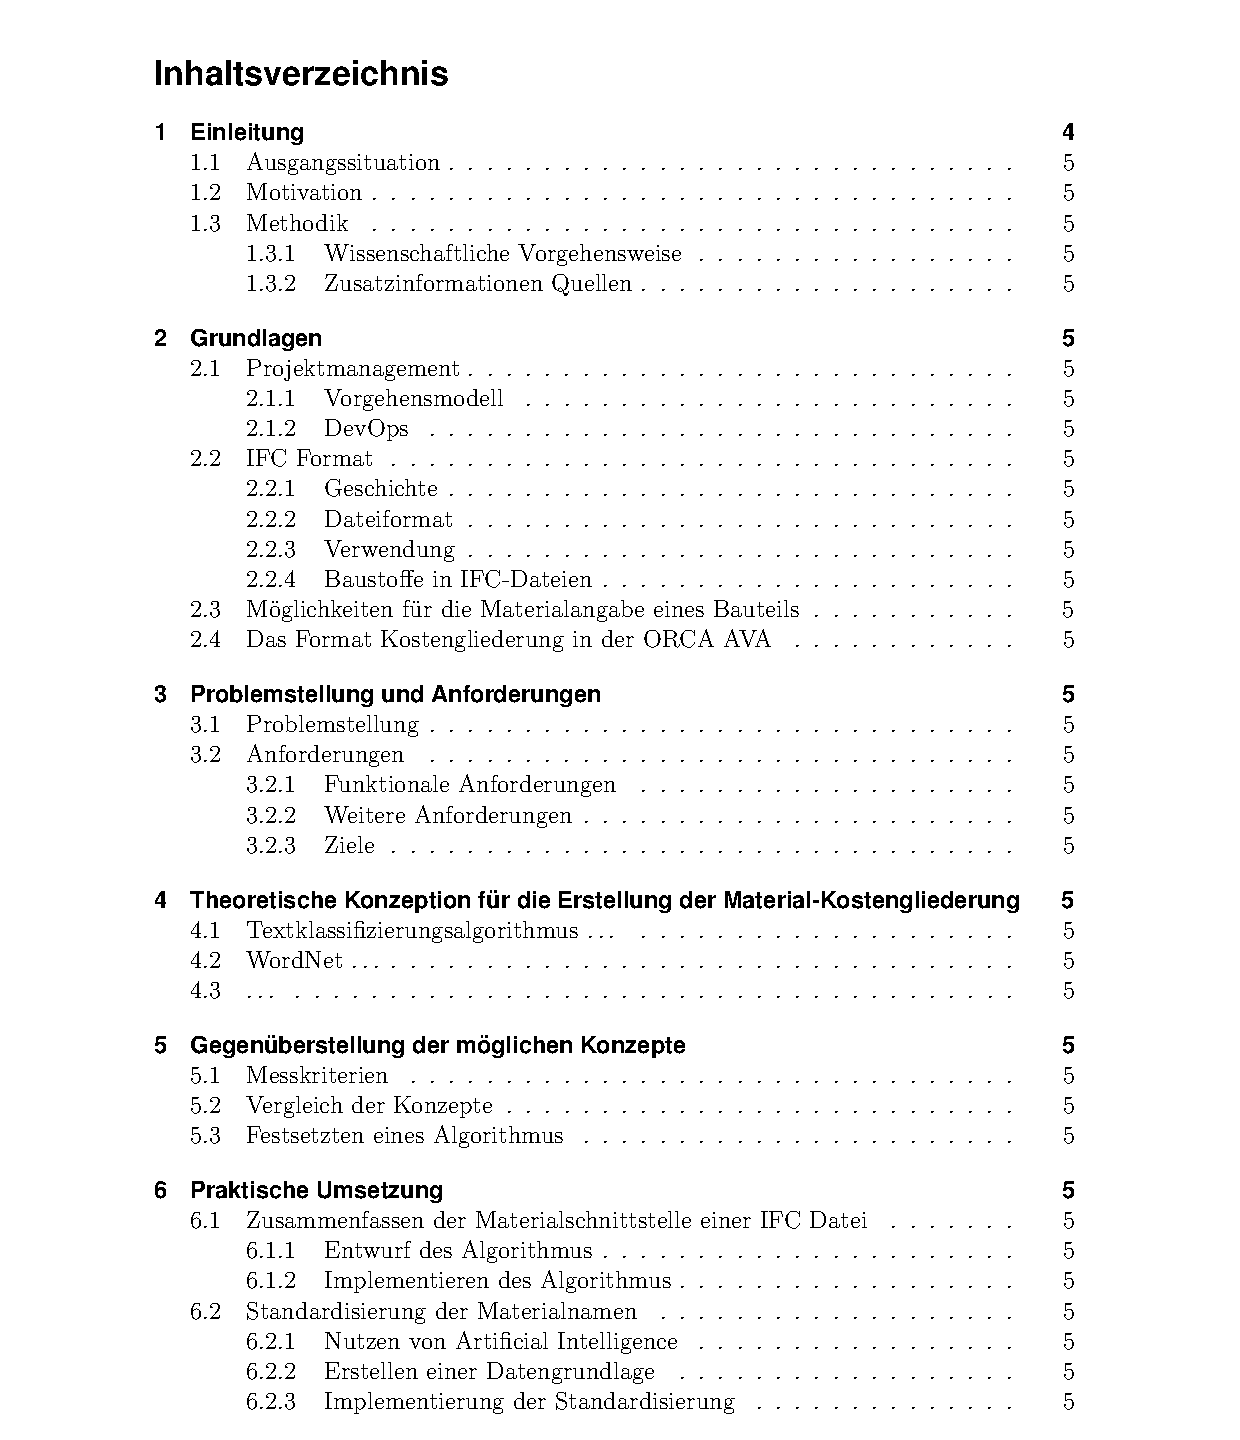
\includepdf[pages=-]{figures/inhaltsverzeichnis.pdf}
\section{Zeitplan}

\begin{description}
	\item[1.]
	Recherchieren über verschiedene mögliche Techniken und Algorithmen (2 Wochen)
	\item[2.] 
	Austesten der gefundenen Algorithmen (2 Wochen)
	\item[3.]
	Messen der Ergebnisse der Algorithmen (1 Wochen)
	\item[4.] Implementieren des besten Ergebnisses (1 Wochen)
	\item[5.] Schreiben der Arbeit (ca. 6 Wochen)
\end{description}

%\section{Erste Literatur}

%Für IFC gibt es von buildingSMART eine technische Beschreibung der Schnittstelle. Diese hilft die möglichen Materialangaben zu lokalisieren und zusammenfügen zu können. \cite{security-model}
\end{onehalfspace}